\chapter{边界环标签下基于半监督自训练的弱监督语义分割}
\section{引言}
\label{sec:boundingring-intro}
% 边界框标签
计算机视觉中,目标检测任务使用边界框作为监督标签,它指的是标注者绘制出目标的外接矩形,使得目标的所有像素都被限定在该矩形中,能够标识出该目标的所在位置、尺寸大小、所属类别等信息。
\figureref{fig:boundingbox-samples}展示了 PASCAL VOC 2012 数据集中三幅图片及它们的边界框标签,其中不同颜色的框对应不同的目标类别。
% 能够用于实例分割
与\chapterref{chp:scribble}中介绍的涂鸦线标签类似,边界框标签也能以较低的标注成本给出目标的大致位置,且与目标实例一一对应的特性还使其能够应用于弱监督实例分割[]等领域。
尽管如此,这种标签之于弱监督语义分割存在以下弱点:
% 边界框标签的难点
\par
(1)\textbf{缺乏可信像素}:
本质上看,语义分割是像素级的分类任务,其模型是在已知大量像素类别的前提下进行的。
比如,以交叉熵作为分割任务的损失,就是将各个像素点视为了分类样本。
然而,边界框仅保证了目标像素不会落在框外,除此之外没有任何额外先验信息,这意味着没有办法确定任何一部分像素的类别。
如\figureref{subfig:boundingbox-sample-1}中“摩托车”这一类别所示,真正属于“摩托车”这一目标的像素都分布在框的对角线上,这一点从框本身出发是无法获知的。
\par
(2)\textbf{对不规则目标的敏感性}:
由于二维图像中存在遮挡、透视等现象,某些在三维空间中形状规则的目标,在二维空间中可能出现像素分布与矩形差异较大的情况,称为不规则目标,具体表现为少量像素以远离分布中心的形式出现在图像中。
对于不规则目标,由于边界框就是目标所有像素点的最小外接矩形,所以这种标签的覆盖范围很容易受到少量不规则像素的影响。
如\figureref{subfig:boundingbox-sample-2}中“马”这一类别,像素呈“L”型分布,导致其边界框几乎占据了整幅图像,相当于所给出的位置信息量非常有限。
\begin{figure}[h]
\centering
\subfloat[]{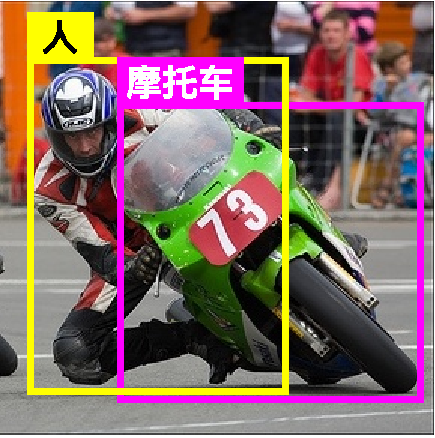
\includegraphics[width=.3\linewidth]{boundingbox-sample-1}%
\label{subfig:boundingbox-sample-1}}
\hfil
\subfloat[]{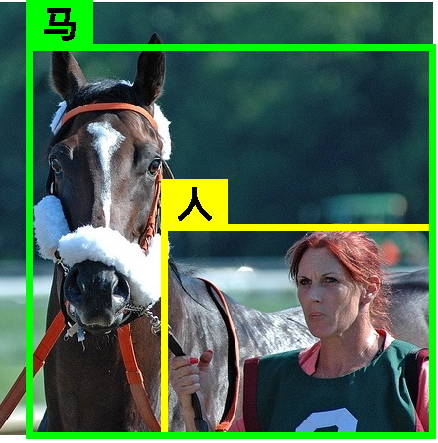
\includegraphics[width=.3\linewidth]{boundingbox-sample-2}%
\label{subfig:boundingbox-sample-2}}
\hfil
\subfloat[]{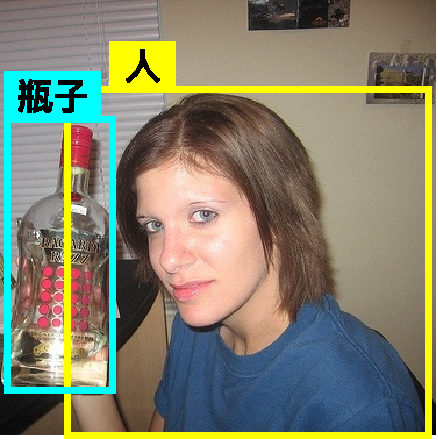
\includegraphics[width=.3\linewidth]{boundingbox-sample-3}%
\label{subfig:boundingbox-sample-3}}
\caption{边界框标签示例}
\label{fig:boundingbox-samples}
\end{figure}
\par
% 难点解决
为了解决以上这些问题,本章节以新提出的边界环标签为研究对象,设计了一种面向街景图像的、基于半监督自训练的弱监督语义分割框架 Weak2Semi。
该框架首先设计了一种基于视觉注意力图的伪标签初始化策略,借助于分类标签不随标注者而变化的特点,规避了线标签的主观性对于模型性能的影响;然后,基于超像素与图卷积算子设计了一个区域相似度建模网络,最后
\section{基于半监督自训练的街景图像弱监督分割框架 Weak2Semi}
\begin{figure}[h]
\centering
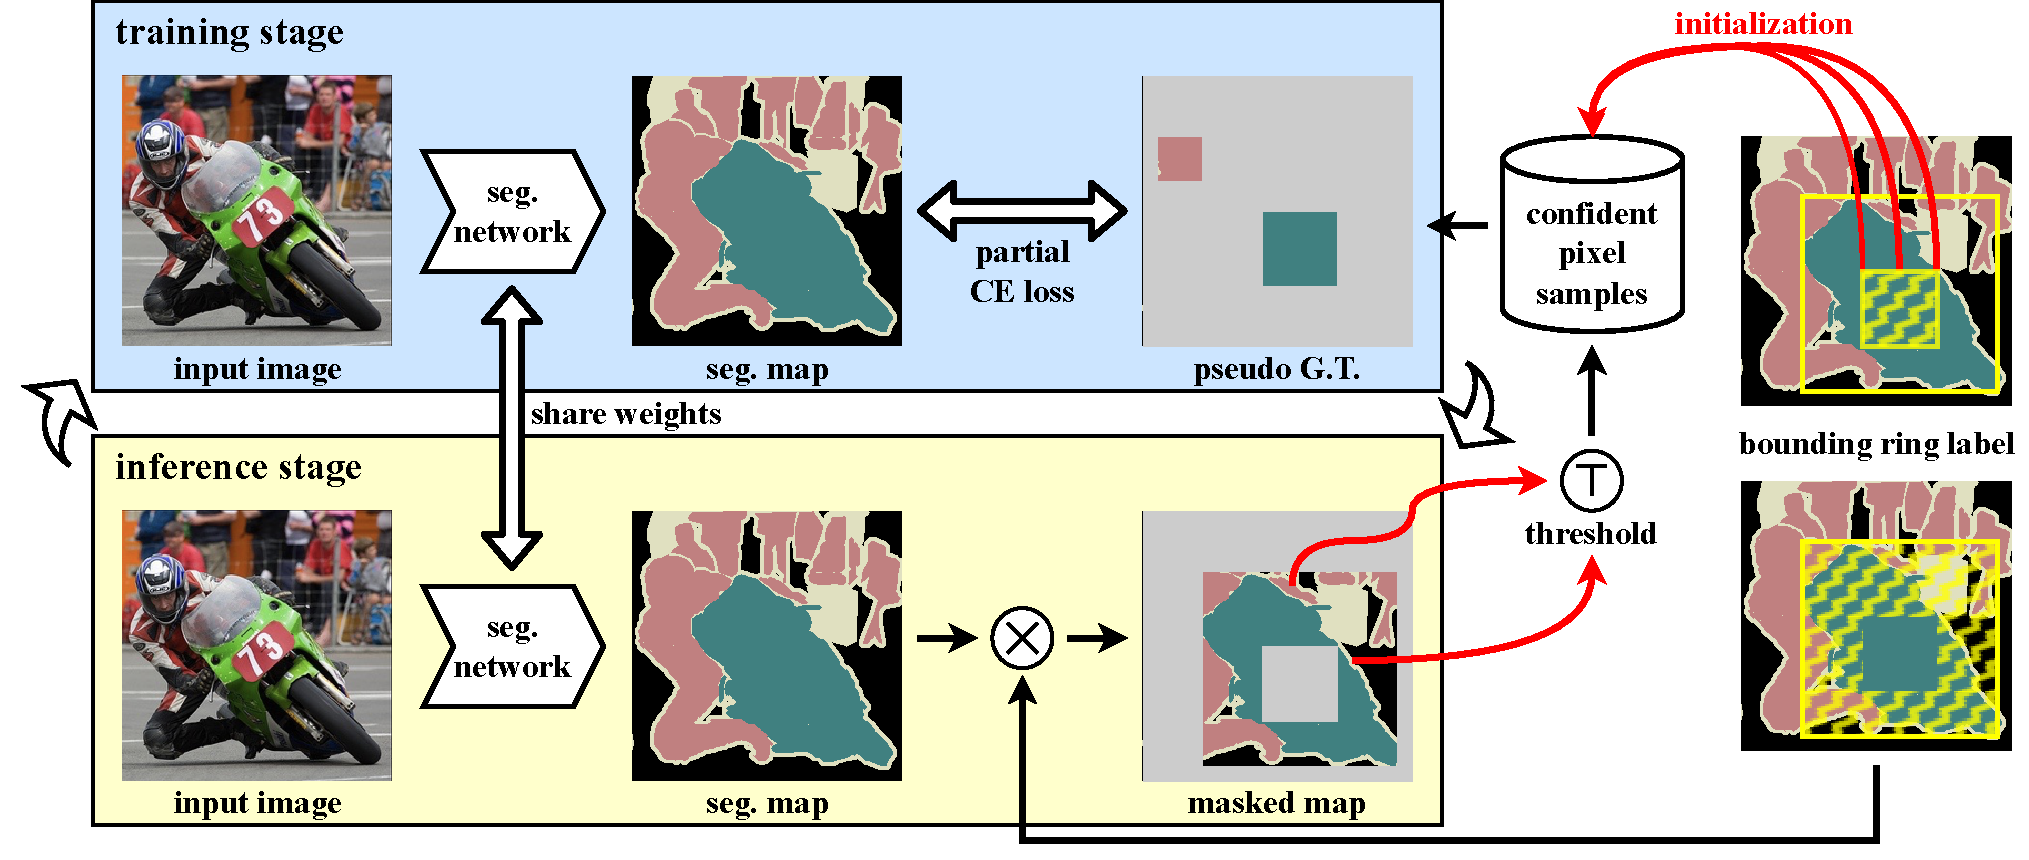
\includegraphics[width=\linewidth]{weak2semi-arch}
\caption{基于半监督自训练的弱监督语义分割框架 Weak2Semi}
\label{fig:weak2semi-arch}
\end{figure}
% 对框架 Weak2Semi 的一段话介绍
Weak2Semi(\textbf{Weak}ly Supervision to \textbf{Semi} Supervision)
\subsection{基于边界环标签的弱监督分割标注形式}
\label{subsec:boundingring}
针对\sectionref{sec:boundingring-intro}中边界框存在的诸多不足,我们在这种标签的基础上提出一种新的弱监督语义分割标注形式:边界环(bounding ring)标签。
顾名思义,环标签由内框和外框两个矩形构成,其中外框是目标的外接矩形(即边界框标签),内框则是目标的内接矩形,如\figureref{fig:boundingring}所示。
% 脚注:(最小)外接矩形、(最大)内接矩形,都是指与坐标轴方向平行的简单矩形,不考虑旋转的情况
外框确保目标所有像素不会落在其外部,内框确保其内部所有像素都属于目标类别。
通常情况下,内外框可以共享中心点,此时我们要求标注者先绘出外接矩形,由标注软件自动确定中心点位置,然后再绘制内接矩形,这一流程省略了确定内接矩形具体位置的步骤,仅需确定其长宽即可。
\begin{figure}[h]
\centering
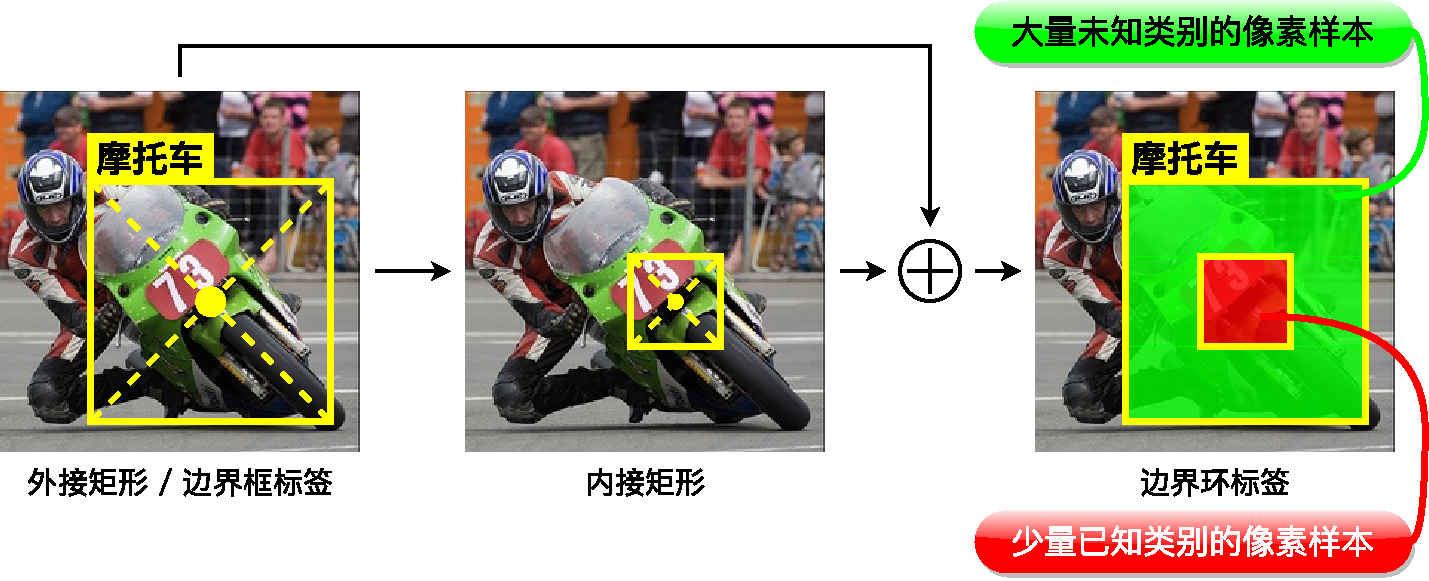
\includegraphics[width=\linewidth]{boundingring}
\caption{边界环标签示例}
\label{fig:boundingring}
\end{figure}
\par
与其他弱监督标注形式相比,边界环标签继承了边界框的优势。
同时,由于边界环仅是在边界框的基础上新增了一个内接矩形,所以可以认为两者具有同一量级的低标注成本(特别是,在内外框共享中心点的情况下,标注操作只增加了一步),相比像素级的分割标签仍是巨大进步。
此外,这一新标签还解决了\sectionref{sec:boundingring-intro}中提出的两个难点:
\par
(1)\textbf{补充了可信像素}:
得益于内接矩形,边界环提供了外框范围内少量像素的类别信息,这一部分像素对于语义分割任务的训练很有帮助。
极端情况下,不设计弱监督学习框架,直接训练全监督模型,并仅以内框内部像素作为前景像素,以外框外部像素作为背景像素,忽略内外框中间像素(下称“环内像素”)的梯度回传,仍能得到精度尚可的语义分割网络,这足以说明少量可信像素的重要性。
同时,这些已知类别像素是二维邻接的,这也有利于卷积神经网络学习空间局部性。
\par
(2)\textbf{感知目标主体位置}:
如\sectionref{sec:boundingring-intro}所述,外框的覆盖范围很受目标不规则程度的影响。
然而,我们在 PASCAL VOC 2012 数据集[]上使用分割标签生成边界环标签(生成算法下述),并对这些生成标签进行统计之后发现,对于不规则目标,其主体像素几乎都落在最大内接矩形的附近,越远离内框的像素越不可能是目标像素。
换句话说,对于内外框面积差距较大的目标,我们不仅能得知该目标是不规则形状的,还能由内框所在位置判断出目标的主体位置。
这一点使得环标签规避了对不规则目标的敏感性,为语义分割任务提供了更有利的先验信息。
\par
% 现有语义分割数据集的分割标签 -> 边界环标签
本文虽然设计的是弱监督下的语义分割框架,但在实际实验过程中所使用的仍是带有像素级分割标签的数据集,只是不直接使用这些全监督标签,而是将这些标签转为各章节所介绍的弱标签进行训练。
这是因为,在模型通过弱监督方法训练完成后,需要这些全监督标签对伪标签质量、模型精度等进行评估,进而比较不同弱监督方法的好坏。
假设语义分割数据集中的某个样本为 $(I, Y^{*})$,其中 $I \in \mathcal{R}^{h \times w}$ 为图像,$Y^{*} \in [0, n^\text{class}-1]^{h \times w}$ 为语义分割标签,其每个元素 $Y^{*}[x,y] = c$ 代表图像在该处属于类别 $c$,下面阐述如何将此全监督标签转化为本章所使用的边界环标签。
\par
边界环标签由外接矩形和内接矩形构成。
在生成过程中,为确保弱标签提供足够多的先验信息,我们限定外接矩形需是能够框住目标的最小外接矩形,内接矩形需是能填充在目标内部的最大内接矩形。
% 多个目标属于同一类别的情况
最小外接矩形的生成算法较显然:遍历属于当前目标的所有像素,记录遍历过程中的最小横坐标 $x_1^\text{ex}$、最大横坐标 $x_2^\text{ex}$、最小纵坐标 $y_1^\text{ex}$、最大纵坐标 $y_2^\text{ex}$,则最小外接矩形 $\text{Rec}_c$ 的左上角坐标是 $(x_1^\text{ex}, y_1^\text{ex})$,右下角坐标是 $(x_2^\text{ex}, y_2^\text{ex})$:
\begin{equation}
\begin{split}
  \text{Rec}^\text{ex}_c = &(x_1^\text{ex}, y_1^\text{ex}, x_2^\text{ex}, y_2^\text{ex})\\
= &(\min(x), \min(y), \max(x), \max(y)),\ \forall Y^{*}[x,y] = c    
\end{split}
\end{equation}
\par
最大内接矩形的生成过程则较为复杂。
基于最小外接矩形所提供的四个坐标,我们定义了一种思想类似于扫描线算法[]的生成算法:
首先,遍历最小外接矩形中的所有像素,将网格形式的分割标签转换为目标像素集合。
接着,使用边缘检测算法,从目标像素集合获得目标轮廓。
然后,使用纵向扫描线遍历最小外接矩形所框区域。
在每轮遍历中,通过交点的方式确定以该扫描线为左边界的内接矩形。
最后,保留面积最大的内接矩形作为答案。
该算法的形式化表示见\algorithmref{alg:in-rec}。
\algrenewcommand\algorithmicrequire{\textbf{输入:}}
\algrenewcommand\algorithmicensure{\textbf{输出:}}
\begin{algorithm}
\caption{最大内接矩形生成算法}
\label{alg:in-rec}
\begin{algorithmic}[1]
\Require $x$
\Ensure $y$
\For {$c = 0, \dots, n^\text{class}-1$}
\State $R_c \gets \varnothing$
\Comment{目标像素集合}
\For {$x = x_1^\text{ex} \dots x_2^\text{ex}$}
\For {$y = y_1^\text{ex} \dots y_2^\text{ex}$}
\If {$Y^{*}[x,y] = c$}
    {$R_c \gets R_c \cup \{(x,y)\}$}
\EndIf
\EndFor
\EndFor
\State $E_c \gets f_\text{edge}(R_c)$
\Comment{边缘检测算法}
\State $x_1^\text{in} \gets 0, x_2^\text{in} \gets 0, y_1^\text{in} \gets 0, y_2^\text{in} \gets 0$
\For {$x_1 = x_1^\text{ex} \dots x_2^\text{ex}$}
\State {求直线 $x = x_1$ 与轮廓的所有交点,并对这些交点按纵坐标倒序排序,取出前两个 $(x_1, y_2)$ 和 $(x_1, y_1)$}
\State {求直线 $y = y_1$ 与轮廓的所有交点,从中找到纵坐标大于 $y_1$ 的最左交点 $x_{2,1}$}
\State {同理,由直线 $y = y_2$ 求出 $x_{2,2}$}
\State {$x_2 = \min(x_{2,1}, x_{2,2})$}
\If {$(x_2 - x_1) \times (y_2 - y_1) > (x_2^\text{in} - x_1^\text{in}) \times (y_2^\text{in} - y_1^\text{in})$}
\State {$x_1^\text{in} \gets x_1, x_2^\text{in} \gets x_2, y_1^\text{in} \gets y_1, y_2^\text{in} \gets y_2$}
\EndIf
\EndFor
\State $\text{Rec}^\text{in}_c = (x_1^\text{in}, y_1^\text{in}, x_2^\text{in}, y_2^\text{in})$
\Comment{最大内接矩形}
\EndFor
\State \Return $\text{Rec}^\text{in}_{0}, \dots, \text{Rec}^\text{in}_{n^\text{class}}$
\end{algorithmic}
\end{algorithm}
\subsection{基于半监督自训练的伪标签像素扩充算法}\label{subsec:semi}
% 弱监督任务 -> 半监督任务
将像素视为一个个的训练样本,则内框内部像素是少量已知类别的样本,环内像素是大量未知类别的样本,此问题就可以由“弱监督语义分割”转化为“半监督图像分类”问题,进而用半监督算法解决。
基于半监督学习中的自训练(self-training)策略,我们提出了一个结合了指数衰减交叉熵损失与空间感知阈值的半监督自训练框架,如\figureref{fig:weak2semi-network}所示。
该框架以内框内部像素为出发点,通过“训练+推理”循环往复的形式,不断扩充伪标签像素。
与\sectionref{subsec:walk}中涂鸦线的情况类似,对此初始伪标签只需考虑漏标的情况,优化伪标签质量的过程就是扩充伪标签面积的过程。
\begin{figure}[h]
\centering
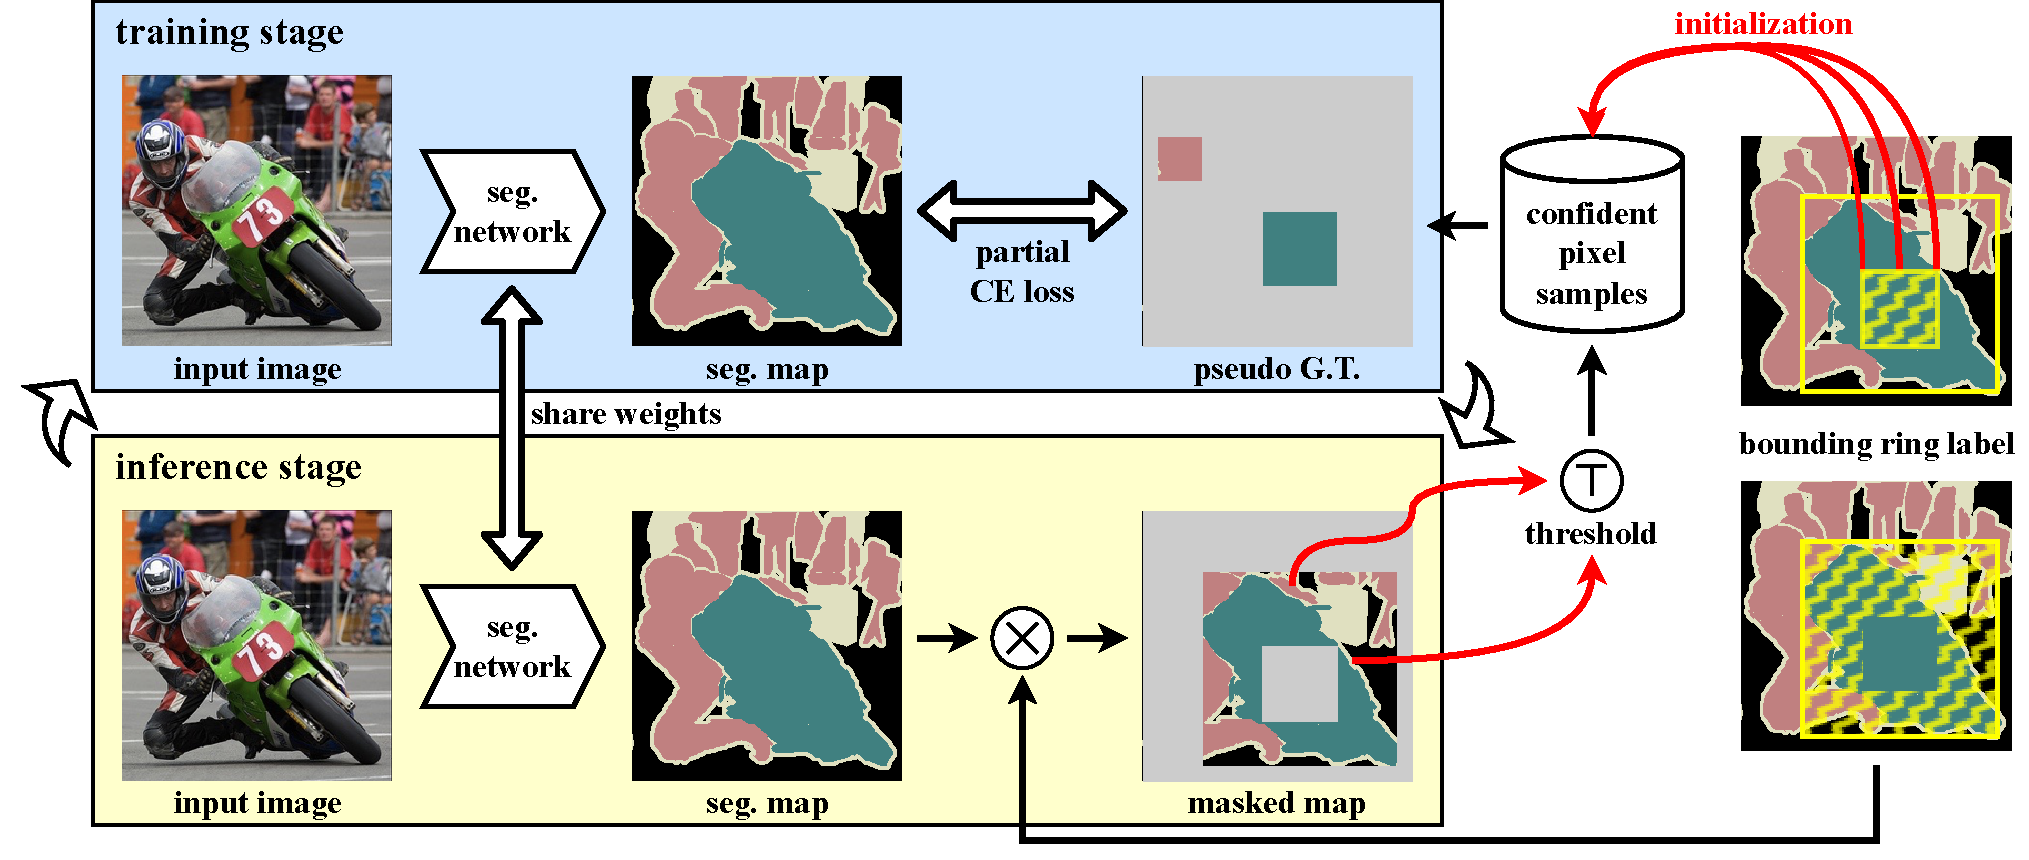
\includegraphics[width=\linewidth]{weak2semi-network}
\caption{基于半监督自训练的弱监督语义分割框架 Weak2Semi}
\label{fig:weak2semi-network}
\end{figure}
\par
% 自训练
具体来说,以像素为样本,对于每个类别 $c$,我们都构建可信样本集合 $S_c = \{(x_1,y_1), (x_2,y_2), \dots\}$,包含本轮迭代中用于训练分割网络的所有像素。
所有未出现在 $S_1, S_2, \dots, S_{n^\text{class}}$ 中的像素将不参与梯度回传,也就不会被用于更新模型参数。
在初始化阶段,可信像素全部来自边界环的内框 $\text{Rec}^\text{in}_c$ 所包围的区域,即:
\begin{equation}
S_c \vert_{t=1} = \{(x,y):\ x \in [x_1^\text{in}, x_2^\text{in}]\ \ \text{and}\ \ y \in [y_1^\text{in}, y_2^\text{in}]\}
\end{equation}
\par
对于第 $t$ 轮迭代($1 \le t \le n^\text{epoch}$),我们将其分为训练和推理两个子步骤。
在训练步骤中,我们的目的是使用新老样本对模型参数进行更新:
首先,将可信样本集合转换为与原图大小一致的掩码图 $\mathbf{M}^\text{fg}_c\vert_t \in \{0,1\}^{h \times w}$,便于后续损失函数的高效计算:
\begin{equation}
\mathbf{M}^\text{fg}_c\vert_{t}[x,y] =
\begin{cases}
1,&\text{if}\ \ (x,y) \in S_c\vert_{t}\\
0,&\text{else}
\end{cases}
\label{eqn:mask-fg}
\end{equation}
\par
接着,假设分割网络对图像的预测结果为 $\mathbf{Y} \in [0,1]^{h \times w \times n^\text{class}}$,我们使用一个局部交叉熵损失,仅计算可信样本与真实类别之间的概率分布差异。
同时,对于不同轮次加入的样本 $(x,y)$,我们采取不同的损失权重 $\mathbf{W}_c\vert_{t}[x,y]$,使得新老样本对于模型参数更新有不同程度的影响力:
\begin{equation}
\mathcal{L} = - \sum\limits_{(x,y)}^{I} \sum\limits_{c=1}^{n^\text{class}} \mathbf{W}_c\vert_{t}[x,y] \mathbf{M}^\text{fg}_c\vert_{t}[x,y] \log{\mathbf{Y}[x,y,c]}
\label{eqn:weighted-crossentropy}
\end{equation}
\begin{equation}
\mathbf{W}_c\vert_{t}[x,y] =
\begin{cases}
\alpha^{t - t^\prime},&\text{if}\ \ (x,y) \in (S_c\vert_{t^\prime}{\setminus}S_c\vert_{t^\prime-1})\\
0,&\text{else}
\end{cases}
\label{eqn:loss-weight}
\end{equation}
通常 $\alpha$ 取 $[0.9, 1)$ 区间内的某个数。
\equationref{eqn:loss-weight}的含义是,对于第 $t^\prime$ 轮新加入的样本 $(x,y) \in (S_c\vert_{t^\prime}{\setminus}S_c\vert_{t^\prime-1})$,其损失权重为超参数 $\alpha$ 的 $t - t^\prime$ 次幂。
对于越早加入的样本,其 $t - t^\prime$ 值越大,进而 $\alpha^{t - t^\prime}$ 越小;反之,越晚加入的样本具有越大的 $\alpha^{t - t^\prime}$ 值。
这意味着,老样本在损失函数中的比重会指数级衰减,新样本将对模型训练起更大作用,这使得模型在每轮训练时更加关注于新样本,与半监督学习的要求相符。
另外,需注意到\equationref{eqn:weighted-crossentropy}不同于一般的交叉熵损失,后者在整幅图片的任意像素上损失值都非 $0$,而前者在集合 $S_c\vert_{t}$ 以外的像素处损失值始终为 $0$。
\par
% 空间感知阈值
使用\equationref{eqn:weighted-crossentropy}对分割网络的参数进行更新后,进入本轮迭代的推理子步骤,该步骤是为了从大量未知类别的样本中筛出高置信度的部分,作为下一轮的训练样本:
首先,筛选出位于环内且未知类别的所有样本,构成未知样本集合 $S^\text{unknown}_c$:
\begin{equation}
S^\text{unknown}_c = \left\{(x,y):\ x \in [x_1^\text{ex}, x_2^\text{ex}]\ \ \text{and}\ \ y \in [y_1^\text{ex}, y_2^\text{ex}]\ \ \text{and}\ \ (x,y) \notin S_c\vert_{t}\right\}
\end{equation}
\par
\begin{figure}[h]
\centering
% \includegraphics[width=\linewidth]{} % 画图(画出各 x 和 y)
\caption{环内空间的八个象限}
\label{fig:8-quadrant}
\end{figure}
如\figureref{fig:8-quadrant}所示,内外框相当于将环内空间划分成了八个象限。
对于不同象限中的未知样本,其与内环的最短距离 $\text{dis}(x,y)$ 有着不同的定义,表述为\equationref{eqn:distance}:
对于四个角上的第 1、3、6、8 象限,该最短距离等于样本与相应对角点的距离;
对于另外的第 2、4、5、7 象限,该最短距离则等于样本与相应矩形边的距离。
\begin{equation}
\text{dis}(x,y) =
\begin{cases}
\sqrt{(x_1^\text{in} - x)^2 + (y_1^\text{in} - y)^2},&\text{if}\ \ x \in [x_1^\text{ex}, x_1^\text{in}]\ \ \text{and}\ \ y \in [y_1^\text{ex}, y_1^\text{in}]\\
y_1^\text{in} - y,&\text{if}\ \ x \in [x_1^\text{in}, x_2^\text{in}]\ \ \text{and}\ \ y \in [y_1^\text{ex}, y_1^\text{in}]\\
\sqrt{(x - x_2^\text{in})^2 + (y_1^\text{in} - y)^2},&\text{if}\ \ x \in [x_2^\text{in}, x_2^\text{ex}]\ \ \text{and}\ \ y \in [y_1^\text{ex}, y_1^\text{in}]\\
x_1^\text{in} - x,&\text{if}\ \ x \in [x_1^\text{ex}, x_1^\text{in}]\ \ \text{and}\ \ y \in [y_1^\text{in}, y_2^\text{in}]\\
x - x_2^\text{in},&\text{if}\ \ x \in [x_2^\text{in}, x_2^\text{ex}]\ \ \text{and}\ \ y \in [y_1^\text{in}, y_2^\text{in}]\\
\sqrt{(x_1^\text{in} - x)^2 + (y - y_2^\text{in})^2},&\text{if}\ \ x \in [x_1^\text{ex}, x_1^\text{in}]\ \ \text{and}\ \ y \in [y_2^\text{in}, y_2^\text{ex}]\\
y - y_2^\text{in},&\text{if}\ \ x \in [x_1^\text{in}, x_2^\text{in}]\ \ \text{and}\ \ y \in [y_2^\text{in}, y_2^\text{ex}]\\
\sqrt{(x - x_2^\text{in})^2 + (y - y_2^\text{in})^2},&\text{if}\ \ x \in [x_2^\text{in}, x_2^\text{ex}]\ \ \text{and}\ \ y \in [y_2^\text{in}, y_2^\text{ex}]\\
\end{cases}
\label{eqn:distance}
\end{equation}
\par
假设带有新参数的语义分割网络对图像的推理结果为 $\mathbf{Y} \in [0,1]^{h \times w \times n^\text{class}}$,那么基于以上最短距离定义,我们提出了一种距离感知的置信度阈值(distance-aware confidence threshold),作为未知样本转变成可信样本的筛选标准:
\begin{equation}
S_c\vert_{t+1} = S_c\vert_{t} \cup \left\{(x,y):\ \mathbf{Y}[x,y,c] > \theta + \cfrac{\text{dis}(x,y)}{\max_{(x,y) \in T_c} \text{dis}(x,y)} (1-\theta)\right\}
\label{eqn:dis-aware-conf-thres}
\end{equation}
通常 $\theta$ 取 $[0.5, 1)$ 区间内的某个数,取值越大意味着整体对像素的筛选更加严格。
\equationref{eqn:dis-aware-conf-thres}的作用是,仅将那些置信度高于某个阈值的样本加入到下一轮的可信样本集合 $S_c\vert_{t+1}$ 中,这一阈值落在 $(\theta, 1)$ 区间内。
若该样本离内框越近,则 $\text{dis}(x,y)$ 将越小,导致阈值越接近于 $\theta$,反之则越接近于 $1$。
这意味着,我们对靠近内框的样本进行宽松的筛选,它们只需较低的置信度就能成为可信样本;对远离内框的样本进行严格的筛选,它们需要较高的置信度才能成为可信样本。
这与\sectionref{subsec:boundingring}所提到的“内框能感知目标主体位置,越远离内框的像素越不可能是目标像素”相符合。
\subsection{基于对比学习的前背景像素特征距离损失}
\begin{figure}[h]
\centering
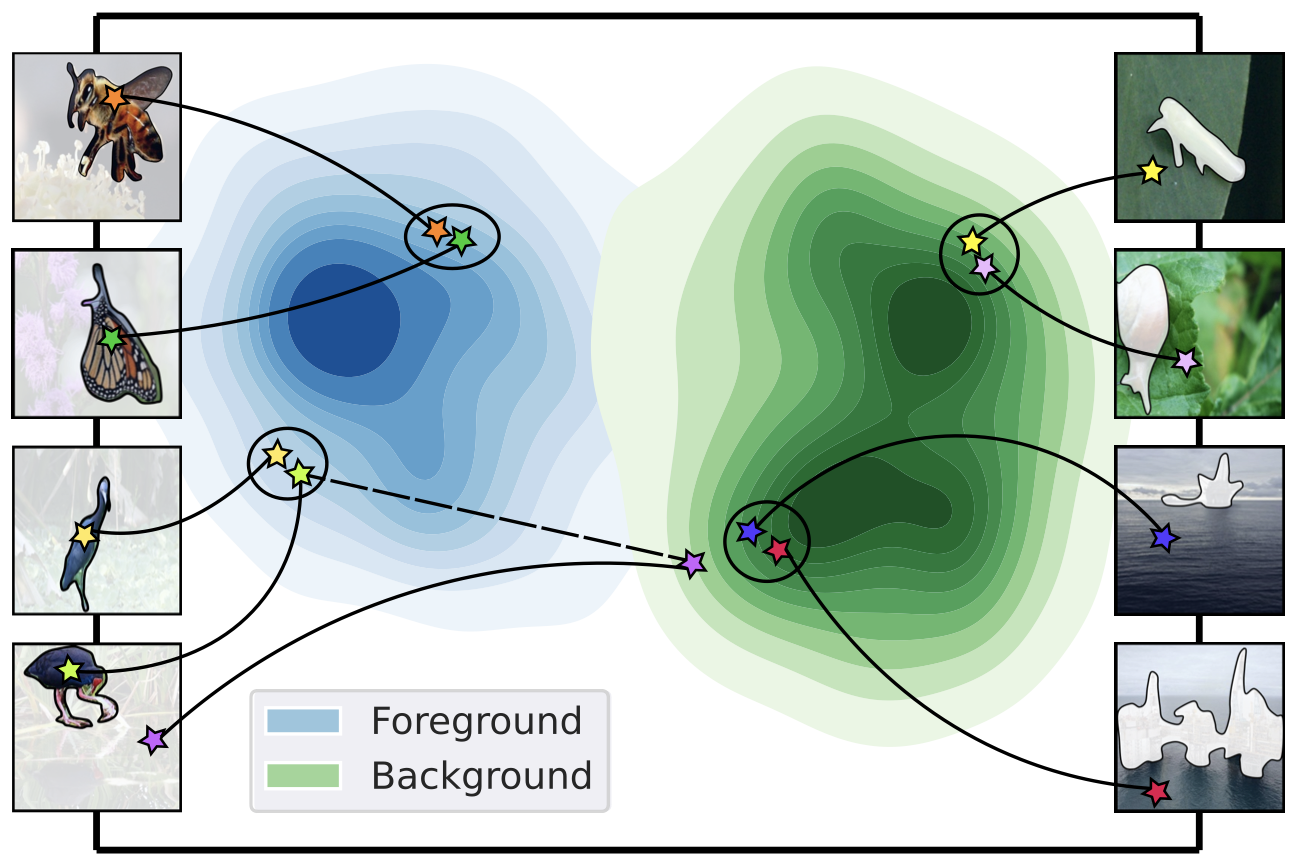
\includegraphics[width=.8\linewidth]{fg-bg}
\caption{不同类别目标的前景像素和背景像素在特征空间中的相对位置}
\label{fig:fg-bg}
\end{figure}
除了使用\equationref{eqn:weighted-crossentropy}中常规的交叉熵损失来训练语义分割网络之外,我们还可以挖掘边界环标签中隐含的更多有用信息。
\figureref{fig:fg-bg}展示了包含不同类别目标的图像,以及这些目标的前景和背景在特征空间中的相对位置。
可以发现以下两点:
(1)对于不同图像中相同类别的多个目标,它们通常具有相似的语义信息,表现为在特征空间中距离较近。
(2)对于同一幅图像中的单个目标,其前景像素和背景像素通常具有各异的语义信息,表现为在特征空间中距离较远。
同时,由\figureref{fig:boundingring}对边界环标签的定义可知,其内框内部像素必定是目标的前景像素(全属于目标类别),外框外部像素必定是目标的背景像素(全不属于目标类别)。
% 脚注:这里的背景像素不一定都属于背景类别,即只是不属于当前类别,可能属于其他类别。
换句话说,边界环标签天然区分出了每个目标的前景像素和背景像素。
因此,借助于边界环天然提供的定位信息,我们可以使用对比学习技术,要求拉近(或拉远)特征空间中的前景向量(或前景向量与背景向量),进而为语义分割网络提供额外监督。
\par
首先,我们考虑如何从输入图像中分别获取前景像素和背景像素。
\equationref{eqn:mask-fg}给出了由可信像素集合生成的前景掩码图 $\mathbf{M}^\text{fg}$,可用于保留输入图像中的前景像素,剔除未知类别像素和背景像素。
类似地,我们构建一张与原图大小同样一致的背景掩码图 $\mathbf{M}^\text{bg}\vert_t \in \{0,1\}^{h \times w}$,其值仅在当前像素位于外框外部时才为 $1$,否则为 $0$:
\begin{equation}
\mathbf{M}^\text{bg}_c\vert_{t}[x,y] =
\begin{cases}
1,&\text{if}\ \ x \in [1, x_1^\text{ex}) \cup (x_2^\text{ex}, w]\ \ \text{or}\ \ y \in [1, y_1^\text{ex}) \cup (y_2^\text{ex}, h]\\
0,&\text{else}
\end{cases}
\label{eqn:mask-bg}
\end{equation}
使用这两个掩码图,通过与输入图像执行逐元素相乘 $\odot$,就能分别得到只保留了前景像素和背景像素的图像(其余位置像素值为 $0$)。
需注意到,由于\sectionref{subsec:semi}半监督框架的存在,前景掩码图中的像素将不断得到扩充,而背景掩码图的像素数量则一直保持不变。
\par
\begin{figure}[h]
\centering
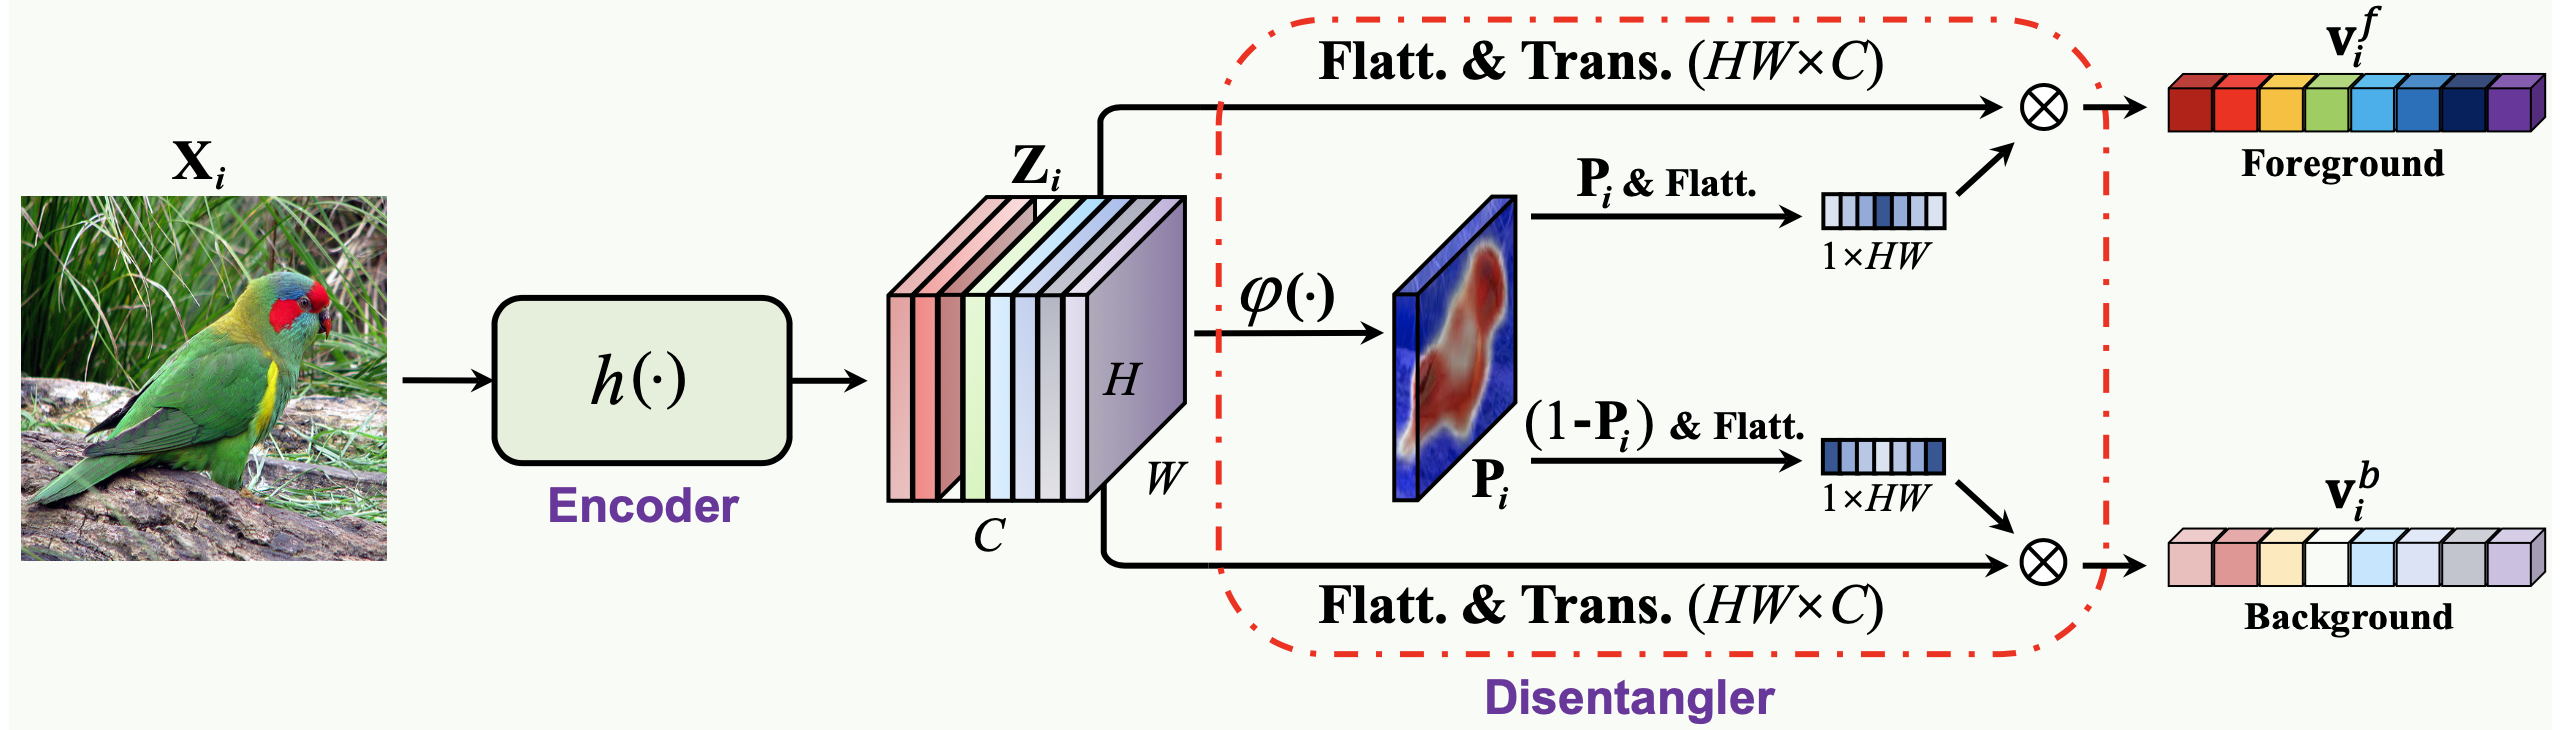
\includegraphics[width=\linewidth]{fg-bg-2-feature}
\caption{}
\label{fig:fg-bg-2-feature}
\end{figure}
接下来,我们考虑如何将这些像素转化为特征向量,为后续对比学习提供比较对象。
基于卷积结构的语义分割网络能够以二维图像为输入,输出一张三维特征图。
假设该特征图的尺寸为 $h^\text{feat} \times w^\text{feat} \times c^\text{feat}$,则其每个像素都是一个长为 $c^\text{feat}$ 的特征向量,共有 $h^\text{feat}w^\text{feat}$ 个这样的像素。
由于对比学习是以两个特征向量作为一个正负例对的,所以这些像素共会产生 $(h^\text{feat}w^\text{feat})^2$ 种组合,在训练过程中将耗费很多的硬件资源。
因此,在此特征图的基础上,我们加入一个全局平均池化层[]将其映射为一维特征向量。
如\figureref{fig:fg-bg-2-feature}所示,对于单张图像中的每个目标,我们生成一个前景特征向量 $\mathbf{v}^\text{fg}_c \in \mathcal{R}^{c^\text{feat}}$ 及一个背景特征向量 $\mathbf{v}^\text{fg} \in \mathcal{R}^{c^\text{feat}}$。
\par
\begin{figure}[h]
\centering
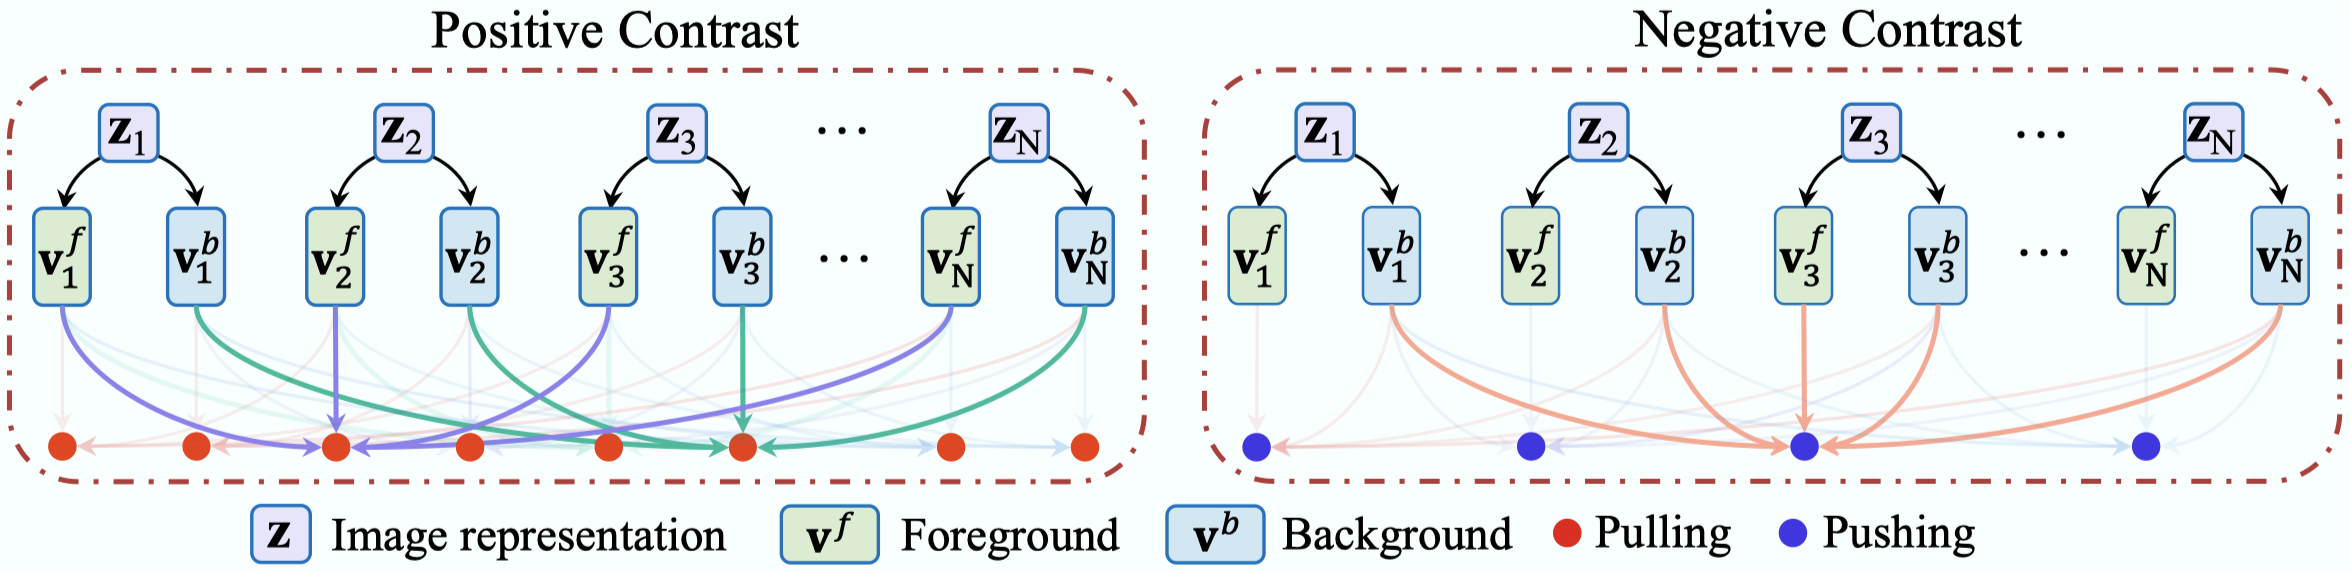
\includegraphics[width=\linewidth]{pos-neg-pairs}
\caption{对比学习中正负例对的构造}
\label{fig:pos-neg-pairs}
\end{figure}
最后,我们构造对比学习中成对的正例或负例,并定义特征空间中的距离损失,作为语义分割网络在交叉熵损失之外的额外监督。
定义两个特征向量 $\mathbf{v}_1$ 和 $\mathbf{v}_2$ 之间的余弦相似度为 $\cos(\mathbf{v}_1, \mathbf{v}_2)$。该相似度越高,代表两个向量在特征空间中的方向越接近:
\begin{equation}
\cos(\mathbf{v}_1, \mathbf{v}_2) = \cfrac{\mathbf{v}_1 \cdot \mathbf{v}_2}{\vert \mathbf{v}_1 \vert \vert \mathbf{v}_2 \vert}
\end{equation}
为了构造足够多的正负例对,我们考虑训练过程中一个批次内的所有 $n^\text{batch}$ 幅图像。
对于每幅图像 $I_i$,我们按照\figureref{fig:fg-bg-2-feature}为所有类别都生成前景特征向量 $\mathbf{v}^\text{fg}_{i,c}, \forall c \in C_i$ 和背景特征向量 $\mathbf{v}^\text{bg}_{i,c}, \forall c \in C_i$,并按照\figureref{fig:pos-neg-pairs}的方式构造正负例对:
(1)对于当前批次不同图像 $I_i, I_j$ 中同一类别 $c$ 的两个前景特征向量 $\mathbf{v}^\text{fg}_{i,c}, \mathbf{v}^\text{fg}_{j,c}$,我们认为它们是正例对,在特征空间中的距离应该拉近,定义对比损失为\equationref{eqn:loss-pos}。
(2)对于同一图像 $I_i$ 中某个类别 $c$ 的前景特征向量 $\mathbf{v}^\text{fg}_{i,c}$ 和背景特征向量 $\mathbf{v}^\text{bg}_{i,c}$,我们认为它们是负例对,在特征空间中的距离应该疏远,定义对比损失为\equationref{eqn:loss-neg}。
\begin{equation}\label{eqn:loss-pos}
\mathcal{L}^\text{pos} = -\cfrac{1}{(n^\text{batch})^2 n^\text{class}} \sum\limits_{i=1}^{n^\text{batch}} \sum\limits_{j=1}^{n^\text{batch}} \sum\limits_{c=1}^{n^\text{class}} 1_{i \neq j} 1_{c \in C_i} 1_{c \in C_j} \log(\cos(\mathbf{v}^\text{fg}_{i,c}, \mathbf{v}^\text{fg}_{j,c}))
\end{equation}
\begin{equation}\label{eqn:loss-neg}
\mathcal{L}^\text{neg} = -\cfrac{1}{n^\text{batch} n^\text{class}} \sum\limits_{i=1}^{n^\text{batch}} \sum\limits_{c=1}^{n^\text{class}} 1_{c \in C_i} \log(1 - \cos(\mathbf{v}^\text{fg}_{i,c}, \mathbf{v}^\text{bg}_{i,c}))
\end{equation}
最终,对比损失被定义为这两者的加和:
\begin{equation}
\mathcal{L}^\text{con} = \mathcal{L}^\text{pos} + \mathcal{L}^\text{neg}
\end{equation}

\section{实验结果与分析}
\subsection{街景图像语义分割数据集 Cityscapes}
街景图像
目标不会叠在一起
有很多目标,可以构造很多正负例对
\subsection{与其他弱监督语义分割算法的比较}

% BFBP:前景背景
% SPN:超像素
% CIAN:跨图片的前景相似度 AAAI'20
% RCA 对比学习

% WSSL & \makecell{ICCV\\2015} 60.6 & 62.2
% BoxSup & \makecell{ICCV\\2015} & 62.0 & 64.2
% SDI 边缘检测算法 HED
% BBAM
% SPML
% A2GNN
% Weakly Supervised Semantic Segmentation via Box-Driven Masking and Filling Rate Shifting

% 全监督:
% DeepLab & 67.6 & 70.3
% ResNet-38 & 80.8 & 82.5

\subsection{针对 Weak2Semi 的消融实验}
\subsection{针对 Weak2Semi 的超参数敏感性分析}
\section{本章小结}
